\documentclass[letterpaper,10pt,twocolumn]{article}
% Layout approximates the AAAI two-column style. For submission, move the body into the AAAI-27 author kit (aaai2027.sty).
\usepackage[letterpaper,top=0.75in,bottom=1.25in,left=0.75in,right=0.75in,columnsep=0.33in]{geometry}
\usepackage{times}
\usepackage{graphicx}
\usepackage{booktabs}
\usepackage{amsmath}
\usepackage{microtype}
\usepackage[font=small,labelfont=bf]{caption}
\setlength{\parskip}{0pt}
\title{\Large\bf Recall, Then Consolidate: Hippocampal Recall Distillation and\\ Selective Replay for Test-Time Memory}
\author{Anonymous submission}
\date{}
\begin{document}
\maketitle
\begin{abstract}
Sliding-window language models with a learned long-term memory, such as Artificial Hippocampus Networks (AHN) and AllMem, write every token into their compressed memory once, when it leaves the window. Complementary Learning Systems (CLS) theory suggests a different division of labour: a fast episodic store keeps experiences exactly, and only what recurs is consolidated, slowly and by replay, into a distributed store. We study SCHEMA, a test-time memory with an episodic store, a slow cortex that changes only through replay, and a replay priority that combines how often an episode is re-used with how much the cortex still gets it wrong. In a controlled associative-memory study, recurrence-weighted consolidation keeps cortex recall near ceiling while error-only priority, arrival-time writes and surprise-scaled writes degrade as one-off events become common ($+0.151$ over error-only priority, 135/135 paired streams); the gap shrinks with cortex capacity, pointing to crowding. On frozen Qwen2.5 models reading fact streams, the decisive ingredient is the write rule: hippocampal recall distillation, which trains the cortex only on episodes the model has actually recalled, consolidates recurring facts without damaging the model, never consolidates one-off facts, and beats the released AHN-GDN-3B by $+0.31$ on our primary score. A pre-registered test on 1.5B shows that SCHEMA's priority beats uniform replay ($+0.039$ [+0.022, +0.056]), but this gain does not replicate on 3B ($-0.010$ [$-0.032$, +0.014]), and an interference gate consistently hurts. We report these negative results as part of the evidence.
\end{abstract}

\section{Introduction}
Hybrid long-context models keep a lossless sliding window and compress what leaves it into a fixed-size memory: a linear recurrent state in AHN \cite{ahn} and a test-time-trained (TTT) nonlinear memory in AllMem \cite{allmem}. Both write at eviction, once and in arrival order. Titans \cite{titans} scales test-time writes by surprise. CLS theory \cite{mcclelland,kumaran} argues that a single store written this way must trade fast acquisition against interference, and that the brain avoids the trade-off with two stores: a hippocampus that encodes episodes at once, and a neocortex that integrates them slowly through interleaved replay. Recent work adds sleep-like phases to language models \cite{lee_sleep,behrouz_sleep} or per-state plasticity \cite{palimpsa}, but consolidates everything that was seen, without asking which experiences deserve it.

We ask a narrower question: \emph{when a test-time memory has an episodic buffer, which episodes should it consolidate?} Our hypothesis, following CLS, is that recurrence, not surprise, should route an experience into slow weights, while one-off surprising events should stay retrievable as episodes. Contributions: (1) SCHEMA, a three-store test-time memory with recurrence-weighted replay; (2) a controlled study, retuned with wide learning-rate grids, that isolates routing, capacity and late-onset regularities; (3) hippocampal recall distillation, a write rule that turns recalled episodes into context-distillation targets; (4) a pre-registered test on a frozen 1.5B model with a 3B replication and a 16k-token run, reporting the parts of the design that failed.

\section{SCHEMA}
\textbf{Stores.} A frozen base attends over a sliding window $W$. Tokens leaving the window are written at once into a \emph{hippocampus} $H$ of key-value landmarks (no gradient step). A \emph{cortex} $C$ (a linear fast-weight matrix in the controlled study, a rank-8 LoRA on the LLM) is read on every step but changed only during periodic micro-sleeps.
\textbf{Tags and routing.} Each episode carries a reuse count $r$ (how often later input re-activated it) and a cortical error $\delta$ (how badly $C$ alone predicts it). At each sleep, episodes with $\delta<\tau$ are released as already consolidated; episodes with $r\geq r_{\min}$ are replayed with probability $\propto \log(1+r)\,\delta$; the rest stay in $H$.
\textbf{Interference gate (optional).} A replay step is accepted only if its gain on the replayed batch exceeds $\rho$ times its damage on a reservoir of anchors, the cortex outputs stored when earlier episodes were consolidated. For a linear cortex both terms have a closed form, and the best step shrinks with the overlap between new and anchor keys.
\textbf{Write rule on an LLM (HRD).} Next-token training on an episode's own text stores the sentence but not an answerable fact \cite{allenzhu}. We therefore use hippocampal recall distillation: when the model reads an $H$ landmark and the stream's next token confirms the copy, the surrounding passage becomes a \emph{recall query} for that episode, and $r$ is the number of confirmed recalls. The cortex is trained so that the model without $H$ matches, at the query, the frozen model that sees the episode in context, a form of context distillation \cite{snell,padmanabhan}. $\delta$ is the remaining KL at the episode's queries. Episodes that are never recalled get no query and are never consolidated.

\begin{figure*}[t]
\centering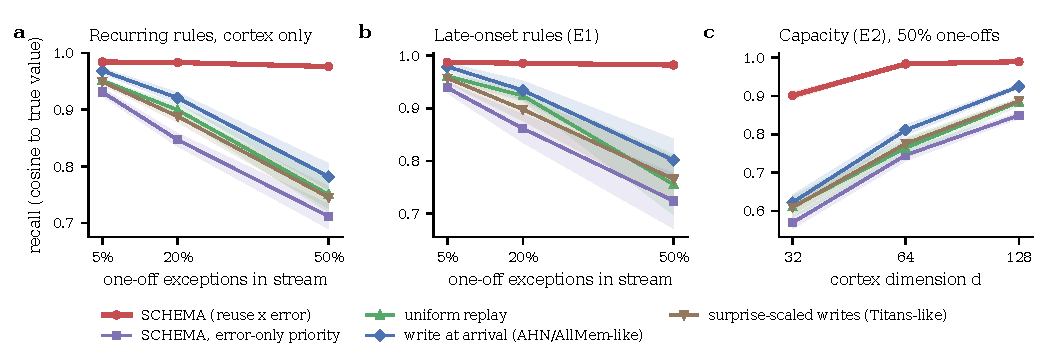
\includegraphics[width=\textwidth]{fig1_stage0a.pdf}
\caption{Controlled study (linear cortex, equal memory bytes, learning rates tuned per arm on validation seeds; 95\% t intervals over seeds). (a) Recall of recurring rules from the cortex alone, averaged over 9 settings of key correlation and rule frequency skew, 5 test seeds each. (b) E1: rules that start mid-stream, so their first occurrence looks like a one-off (10 seeds). (c) E2: cortex dimension $d$ at 50\% one-off events (10 seeds).}
\label{fig:stage0a}
\end{figure*}

\section{Controlled study}
\textbf{Setup.} Streams of $T=2{,}400$ chunks of 4 key-value pairs in $d=64$ dimensions. 32 rules recur with Zipf frequencies; one-off exceptions appear at rate 5, 20 or 50\%, with keys correlated with a rule key (cosine 0, 0.3, 0.6); 25\% of rules change value mid-stream. All arms hold the same bytes (window, $H$, anchors). Baselines: writes at arrival into $C$ with an exact window of equal bytes (AHN/AllMem-like), the same with surprise-scaled steps (Titans-like), sleep over the whole buffer then clear it (sleep-like \cite{lee_sleep}), and uniform replay. Each arm's step size was chosen on validation seeds 0 to 2 from grids of 6 to 7 values; only the sleep-all baseline ended at the edge of its grid. Results use 27 settings $\times$ 5 test seeds (135 paired streams).

\textbf{Recurrence routing protects the cortex.} SCHEMA's cortex recalls recurring rules at 0.98 at every exception rate (Fig.~\ref{fig:stage0a}a). The same system with error-only priority loses $+0.151$ [+0.134, +0.170] (positive on 135/135 streams), and the gap grows with the exception rate ($+0.05$, $+0.14$, $+0.27$). SCHEMA also beats surprise-scaled writes ($+0.120$ [+0.104, +0.138]), arrival writes ($+0.091$ [+0.074, +0.108]) and uniform replay ($+0.114$ [+0.096, +0.133]).
\textbf{Late-onset regularities are consolidated once they recur (E1).} A rule whose first occurrence looks exactly like a one-off is still consolidated (0.98 at all rates, Fig.~\ref{fig:stage0a}b), $+0.143$ [+0.110, +0.180] over error-only priority (30/30 streams).
\textbf{The cost of surprise is crowding (E2).} The gap to error-only priority barely depends on key correlation, and it shrinks as the cortex grows ($+0.33$, $+0.24$, $+0.14$ for $d=32$, 64, 128 at 50\% exceptions; Fig.~\ref{fig:stage0a}c). Consolidating surprising one-offs spends limited cortex capacity and replay budget on items that never return.
\textbf{Episodes and budget.} SCHEMA keeps exceptions 64 to 256 chunks old far better than arrival writes ($+0.347$), but at 50\% exceptions its anchor reservoir takes bytes that uniform replay spends on episodes ($-0.077$ overall). Shrinking the reservoir from 256 to 64 pairs returns those bytes without any cost to the cortex ($+0.001$) and beats uniform replay on exceptions ($+0.101$ [+0.082, +0.120]).
\textbf{The gate does not change recall.} With or without it, cortex recall differs by less than 0.002; it lowers anchor damage slightly (0.010). Reconsolidating anchors when a rule changes matters more: without it the old value lingers ($+0.111$ cosine to the stale value).

\begin{figure*}[t]
\centering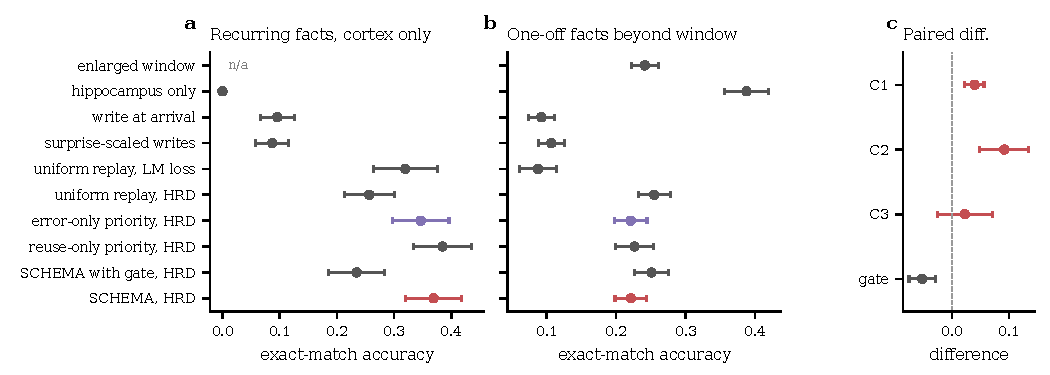
\includegraphics[width=\textwidth]{fig2_neural.pdf}
\caption{Frozen Qwen2.5-1.5B-Instruct, 40 fresh test streams of 8,192 tokens, window 1,024, equal memory bytes and equal replay compute. (a) Exact-match recall of recurring facts after the window and $H$ are cleared (cortex only). (b) Recall of one-off facts more than $W$ tokens back. (c) Pre-registered paired differences with 95\% bootstrap CIs: C1 and C2 on the primary score, C3 on cortex-only recall; ``gate'' is SCHEMA with minus without the gate.}
\label{fig:neural}
\end{figure*}

\section{Frozen-LLM study}
\textbf{Setup.} A frozen Qwen2.5-1.5B-Instruct \cite{qwen} reads 8,192-token streams of facts about invented people (16 recurring facts with paraphrases, one-off facts at rate 20 or 50\%, a quarter of values changed mid-stream) between wikitext-103 passages; 74\% of tokens are filler. Questions are asked after the stream with memory writes disabled, and scored by exact match. Every arm holds the window plus 2,048 key-value pairs per layer and KV head; the LoRA cortex is charged against this budget, and all replay arms take 8 steps every 4 chunks. The \emph{primary score} is the mean of cortex-only recall of recurring facts and recall of one-off facts beyond the window. Settings were tuned on validation seeds 0 to 2 only; the arms, tests and decision rules were written down before the test run on 40 never-used streams (seeds 120 to 139). The no-gate SCHEMA arm was first seen in an earlier exploratory run, which is why we tested it again on fresh streams.

\textbf{Results} (Table~\ref{tab:neural}, Fig.~\ref{fig:neural}). The episodic store alone answers 39\% of one-off facts beyond the window, against 24\% for a window enlarged by the same bytes and 0\% for the window. Recall distillation consolidates recurring facts into the cortex (0.37 cortex-only recall for SCHEMA) without damaging the model (held-out text NLL 2.42, against 4.08 for next-token LoRA replay) and never consolidates one-off facts (cortex-only recall of one-offs is 0 for every distillation arm). Pre-registered tests: \textbf{C1}, SCHEMA beats uniform replay with the same write rule, $+0.039$ [+0.022, +0.056], 33 of 40 streams: \emph{pass}. It stores more recurring facts ($+0.112$ cortex-only recall) and loses a little on one-offs ($-0.034$). \textbf{C2}, it beats uniform next-token replay, $+0.091$ [+0.048, +0.134]: \emph{pass}. \textbf{C3}, reuse-weighted priority beats error-only priority on cortex recall: $+0.022$ [$-0.025$, +0.071]: \emph{fail}. The gate lowers the primary score by $0.052$ [0.030, 0.075] (30 of 40 streams) and costs four times the compute.

\textbf{Scale and length} (Table~\ref{tab:scale}, not pre-registered). On Qwen2.5-3B-Instruct, with step sizes re-tuned on validation seeds, all distillation arms reach about 0.3 on the primary score and beat the released AHN-GDN-3B \cite{ahn}, which recalls 0.5\% of one-off facts beyond the window ($+0.312$ [+0.282, +0.343] for SCHEMA, 40 of 40 streams), and the episodic store alone ($+0.131$). But SCHEMA no longer beats uniform replay ($-0.010$ [$-0.032$, +0.014]) or error-only priority ($+0.018$ [$-0.007$, +0.042]). On 16k-token streams with the 1.5B model, SCHEMA again stores more recurring facts than uniform replay ($+0.079$ [+0.038, +0.122]) and fewer one-offs ($-0.041$), for a primary-score difference of $+0.019$ [$-0.004$, +0.043], and ties error-only priority.

\begin{table}[t]
\centering\small
\caption{Frozen Qwen2.5-1.5B, 40 test streams (means). Cortex: recall of recurring facts with window and $H$ cleared. Beyond W: one-off facts more than $W$ tokens back. NLL: held-out text with the final cortex.}
\label{tab:neural}
\footnotesize\setlength{\tabcolsep}{3pt}
\begin{tabular}{@{}lcccc@{}}
\toprule
arm & prim. & cortex & beyond $W$ & NLL\\
\midrule
Enlarged window & 0.121 & n/a & 0.241 & base\\
Episodic store & 0.194 & 0.000 & 0.388 & base\\
LoRA, at arrival & 0.094 & 0.096 & 0.092 & 2.407\\
LoRA, surprise-scaled & 0.097 & 0.087 & 0.107 & 2.365\\
LoRA, uniform replay & 0.204 & 0.320 & 0.088 & 4.078\\
HRD, uniform replay & 0.256 & 0.257 & 0.255 & 2.381\\
HRD, error-only pri. & 0.284 & 0.347 & 0.221 & 2.420\\
HRD, reuse-only pri. & 0.306 & 0.385 & 0.226 & 2.415\\
HRD, SCHEMA + gate & 0.243 & 0.235 & 0.251 & 2.391\\
\textbf{HRD, SCHEMA} & 0.295 & 0.369 & 0.221 & 2.418\\
\bottomrule
\end{tabular}
\end{table}

\begin{table}[t]
\centering\small
\caption{Scale and length (means). 3B: Qwen2.5-3B, 8k tokens, 40 streams. 16k: Qwen2.5-1.5B, 16k tokens, 20 streams. P: primary; C: cortex-only recurring facts; B: one-offs beyond W.}
\label{tab:scale}
\footnotesize\setlength{\tabcolsep}{2.2pt}
\begin{tabular}{@{}lcccccc@{}}
\toprule
& \multicolumn{3}{c}{3B} & \multicolumn{3}{c}{16k}\\
arm & P & C & B & P & C & B\\
\midrule
Episodic store & 0.189 & 0.000 & 0.377 & 0.108 & 0.000 & 0.217\\
AHN-GDN-3B & 0.007 & 0.009 & 0.005 &  &  & \\
HRD, uniform & 0.329 & 0.379 & 0.279 & 0.243 & 0.361 & 0.124\\
HRD, error-only & 0.301 & 0.307 & 0.296 & 0.264 & 0.443 & 0.085\\
\textbf{HRD, SCHEMA} & 0.319 & 0.349 & 0.289 & 0.262 & 0.441 & 0.084\\
\bottomrule
\end{tabular}
\end{table}

\section{Discussion and limitations}
The robust finding is about \emph{how} a test-time memory should write into slow weights: train the cortex only on what the episodic store has been seen to recall, and distil the model's own in-context behaviour rather than its next-token loss. Distillation arms beat every non-distillation memory we ran at both scales and at 16k tokens, including the trained AHN compressor (next-token LoRA baselines were run at 1.5B only). The CLS-style \emph{selection} story is weaker on LLMs than in simulation. In simulation, recurrence routing beats error routing because one-offs crowd a small cortex; on an LLM, recall distillation already filters out one-offs (an episode that is never recalled gets no query), so the error-only ablation also consolidates only recurring episodes, and C3 becomes a weak test. Reuse-weighted priority shifts capacity from one-off to recurring facts at 1.5B, but on 3B, where the cortex has more room, uniform replay of recalled episodes does as well, consistent with the crowding account from E2. The interference gate, one of our three design principles, did not earn its cost in either study. The prioritized HRD arms beat arrival and surprise-scaled LoRA writes by 0.25 to 0.29 on cortex recall (uniform HRD by about 0.16), but those baselines also use a different write loss. Limitations: one model family and synthetic fact streams; small scale (8k to 16k tokens, up to 3B); and a training-free landmark selector as the episodic store rather than AHN's trained compressor.

{\small
\begin{thebibliography}{99}\setlength{\itemsep}{0pt}
\bibitem{ahn} Y.~Fang, W.~Yu, S.~Zhong, Q.~Ye, X.~Xiong, L.~Wei. Artificial Hippocampus Networks for Efficient Long-Context Modeling. ICML 2026; arXiv:2510.07318.
\bibitem{allmem} Z.~Wang, X.~Wang, K.~Peng, et al. AllMem: A Memory-centric Recipe for Efficient Long-context Modeling. arXiv:2602.13680, 2026.
\bibitem{titans} A.~Behrouz, P.~Zhong, V.~Mirrokni. Titans: Learning to Memorize at Test Time. arXiv:2501.00663, 2024.
\bibitem{mcclelland} J.~L.~McClelland, B.~L.~McNaughton, R.~C.~O'Reilly. Why there are complementary learning systems in the hippocampus and neocortex. Psychological Review 102(3), 1995.
\bibitem{kumaran} D.~Kumaran, D.~Hassabis, J.~L.~McClelland. What learning systems do intelligent agents need? Trends in Cognitive Sciences 20(7), 2016.
\bibitem{lee_sleep} S.~Lee, S.~McLeish, et al. Do Language Models Need Sleep? Offline Recurrence for Improved Online Inference. arXiv:2605.26099, 2026.
\bibitem{behrouz_sleep} A.~Behrouz, et al. Language Models Need Sleep: Learning to Self-Modify and Consolidate Memories. arXiv:2606.03979, 2026.
\bibitem{palimpsa} Learning to Remember, Learn, and Forget in Attention-Based Models (Palimpsa). arXiv:2602.09075, 2026.
\bibitem{allenzhu} Z.~Allen-Zhu, Y.~Li. Physics of Language Models: Part 3.1, Knowledge Storage and Extraction. ICML 2024.
\bibitem{snell} C.~Snell, D.~Klein, R.~Zhong. Learning by Distilling Context. arXiv:2209.15189, 2022.
\bibitem{padmanabhan} S.~Padmanabhan, Y.~Onoe, M.~Zhang, G.~Durrett, E.~Choi. Propagating Knowledge Updates to LMs Through Distillation. NeurIPS 2023.
\bibitem{qwen} Qwen Team. Qwen2.5 Technical Report. arXiv:2412.15115, 2024.
\end{thebibliography}}
\end{document}
